%template1.tex
%The following LaTeX source file represents the simplest kind of slide presentation; no overlays, no included graphics. Substitute your favorite style for ``pascal''. To create the PDF file template1.pdf, (1) be sure to use the prosper class, then (2) execute the command latex template1.tex, and (3) the command dvipdf template1.dvi.

%%%%%%%%%%%%%%%%%%%%%%%%%%%%%%% template1.tex %%%%%%%%%%%%%%%%%%%%%%%%%%%%%%%%%%%
\documentclass[a4paper,blends,pdf,colorBG,slideColor]{prosper}
% definitions for slides for CSC544
% Lutz Hamel, (c) 2007

\hypersetup{pdfpagemode=FullScreen}

\usepackage{times}
\usepackage{latexsym}
\usepackage{alltt}
\usepackage{booktabs}
\usepackage{amsmath}
\usepackage{amsopn}
\usepackage{amsfonts}
\usepackage{amssymb}
%\usepackage[usenames]{color}

\def\sign{\qopname\relax{no}{sign}}
\def\argmax{\qopname\relax{no}{argmax}}
\def\argmin{\qopname\relax{no}{argmin}}

\newcommand{\grad}{\ensuremath{\nabla}} 
\newcommand{\loss}{\ensuremath{{\cal L}}}
\newcommand{\err}{\mbox{err}}
\newcommand{\mse}{\mbox{mse}}
\newcommand{\acc}{\mbox{acc}}
\newcommand{\Integer}{\ensuremath{\mathbb{N}}}
\newcommand{\size}[1]{{|{#1}|}}
\newcommand{\Rnspace}[1]{\ensuremath{\mathbb{R}^{#1}}}
\newcommand{\Real}{\ensuremath{\mathbb{R}}}
\newcommand{\mytt}[1]{{\small\tt{#1}}}
\newcommand{\textemph}[1]{{\em #1}}
\newcommand{\suchthat}{\mid}
\newcommand{\orbar}{\;|\;}
\newcommand{\bs}[1]{\begin{slide}{#1}\ptsize{8}}
\newcommand{\es}{\end{slide}}
\newcommand{\co}{\,\colon\;}
\newcommand{\pair}[2]{\ensuremath{( {#1}, {#2} )}}
\newcommand{\model}[1]{\hat{#1}}
\newcommand{\ul}[1]{{\bf\em #1}}
\newcommand{\ol}{\overline}
\newcommand{\definition}[1]{{\bf Definition: }{\em #1}}
\newcommand{\example}[1]{{\bf Example: }{#1}}
\newcommand{\abs}[1]{|{#1}|}
\newcommand{\mytab}{\makebox[.1in]{}}

\newcommand{\fdef}[1]{
\begin{center}
\fbox{
\begin{minipage}{3.5in}
{\bf Definition:}
{#1}
\end{minipage}
}
\end{center}
}

\newcommand{\fframe}[1]{
\begin{center}
\fbox{
\begin{minipage}{3.5in}
{#1}
\end{minipage}
}
\end{center}
}

\newcommand{\nframe}[1]{
\begin{center}
\begin{minipage}{3.5in}
{#1}
\end{minipage}
\end{center}
}

\newenvironment{Rcode}
	{
		\scriptsize
		\begin{quote}
		\begin{alltt}
	}
	{
		\end{alltt}
		\end{quote}
	}




\begin{document}

\bs{SVMs via Convex Hulls}
Instead of developing SVMs via Langrangian optimization theory we can develop SVM using convex hulls.
\end{slide}

\bs{Convex Hulls}

Let $X =\{ \ol{x}_1, \ol{x}_2,\ldots,\ol{x}_l \} \subset \Rnspace{n}$, then the convex hull of $X$  is the set of all convex combinations of its points, $H(X)$. In a convex combination, each point  in  is assigned a weight or coefficient  in such a way that the coefficients are all non-negative and sum to one, and these weights are used to compute a weighted average of the points. For each choice of coefficients, the resulting convex combination is a point in the convex hull, and the whole convex hull can be formed by choosing coefficients in all possible ways. Expressing this as a single formula, the convex hull is the set:
\[
H(X) = \{ \sum_{i=1}^l \alpha_i\ol{x}_i\}
\]
with $\sum_{i=1}^l\alpha_i = 1$ and $\alpha_i \ge 0$.
\begin{center}
\includegraphics[height=30mm]{images/hull-1.eps}
\end{center}

\es

\bs{SVM: The Separable Case}
Let $D = \{(\ol{x}_1,y_1),\ldots,(\ol{x}_l,y_l)\} \subset \Rnspace{n}\times \{+1,-1\}$ be our training data.
Consider two class distributions +1 and -1 and their corresponding hulls $H(+1)$ and $H(-1)$,
\begin{center}
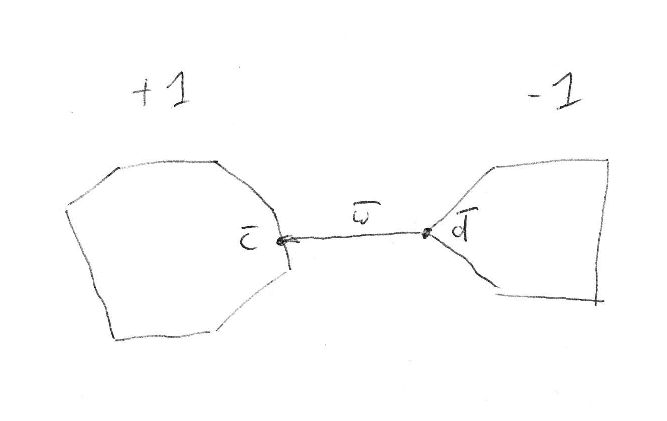
\includegraphics[height=25mm]{images/hull-2.eps}
\end{center}
We pick the point $\ol{c}\in H(+1)$ to be closest to the -1 class distribution and we pick point $\ol{d}\in H(-1)$ to be closest to the +1 distribution.
Next we draw a vector from $\ol{d}$ to $\ol{c}$ such that
\[
\ol{w} = \ol{c} - \ol{d}
\]
Now, picking the points $\ol{c}$ and $\ol{d}$ as we did above and then drawing the vector $\ol{w}$ is the same as saying that we want to minimize
the length of $\ol{w}$, in other words,
\[
\min |\ol{w}| = \min \frac{1}{2} |\ol{w}|^2 = \min \frac{1}{2} \ol{w}\bullet\ol{w}
\]
\es

\bs{SVM: The Separable Case}
Now consider that $\ol{c}\in H(+1)$ and $\ol{d}\in H(-1)$, therefore
\begin{eqnarray*}
\ol{c} &=& \sum_{\ol{x}_p \in +1} \alpha_p^+ \ol{x}_p\\
\ol{d} &=& \sum_{\ol{x}_q \in -1} \alpha_q^- \ol{x}_q
\end{eqnarray*}
Now, let $\ol{\alpha}$ be the {\em concatenation} of $\ol{\alpha}^+$ and $\ol{\alpha}^-$with
\[
|\ol{\alpha}| = |\ol{\alpha}^+| + |\ol{\alpha}^-| = l
\]
then
\[
\min_\alpha \frac{1}{2} \ol{w}\bullet\ol{w} = \min_\alpha \frac{1}{2} \sum_{i=1}^l\sum_{j=1}^l y_i y_j \alpha_i \alpha_j \ol{x}_i \bullet \ol{x}_j
\]
subject to 
\begin{eqnarray*}
\sum_{i=1}^{l} y_i \alpha_i &=& 0 \\
\alpha_i &\ge& 0
\end{eqnarray*}

\es

\bs{SVM: The Separable Case}

It is worthwhile to take a look at the constraint
\[
\sum_{i=1}^{l} y_i \alpha_i = 0
\]
We can rewrite this constraint as
\begin{eqnarray*}
 \sum_{i=1}^{|\ol{\alpha}^+|} (+1) \alpha_i^+ + \sum_{i=1}^{ |\ol{\alpha}^-|} (-1) \alpha_i^- &=& 
 		 \sum_{i=1}^{|\ol{\alpha}^+|}  \alpha_i^+ - \sum_{i=1}^{ |\ol{\alpha}^-|}  \alpha_i^-\\
	&=&	1 - 1\\
	&=& 0 \mbox{  (if the points fulfill the convex hull property)}
 \end{eqnarray*}

\es
\bs{SVM: The Separable Case}

Finally, we have
\[
\max_\alpha - \frac{1}{2}\sum_{i=1}^l\sum_{j=1}^l y_i y_j \alpha_i \alpha_j \ol{x}_i \bullet \ol{x}_j
\]
subject to 
\begin{eqnarray*}
\sum_{i=1}^{l} y_i \alpha_i &=& 0\\
\alpha_i &\ge& 0
\end{eqnarray*}

It is interesting to note that this looks very similar to the optimization problem that we derived via Lagrangian optimization theory.
\es

\bs{SVM: The Non-Separable Case}
\begin{center}
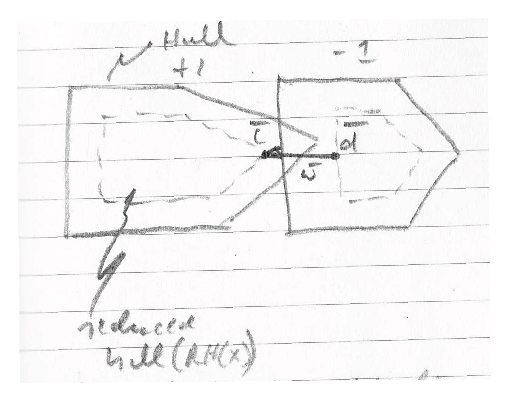
\includegraphics[height=30mm]{images/hull-3.eps}
\end{center}

The {\em reduced hull} $RH(X)$ is defined as
\[
RH(X) = \{ \sum_{i=1}^l \alpha_i\ol{x}_i\}
\]
with 
\begin{eqnarray*}
\sum_{i=1}^l\alpha_i = 1\\
C \ge \alpha_i \ge 0
\end{eqnarray*}

Here we limit the hull multipliers by some cost constant $C$.
\es

\bs{SVM: The Non-Separable Case}

The optimization problem then becomes

\[
\max_\alpha - \frac{1}{2}\sum_{i=1}^l\sum_{j=1}^l y_i y_j \alpha_i \alpha_j \ol{x}_i \bullet \ol{x}_j
\]
subject to 
\begin{eqnarray*}
\sum_{i=1}^{l} y_i \alpha_i = 0\\
C \ge \alpha_i \ge 0
\end{eqnarray*}


\es

\bs{Model}

\begin{center}
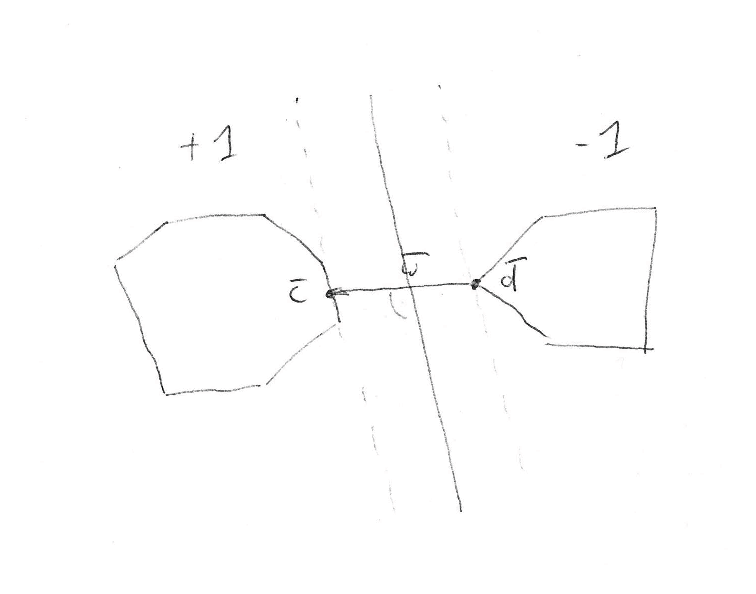
\includegraphics[height=30mm]{images/hull-4.eps}
\end{center}

It is easy to show that our model is a support vector machine,
\[
\model{f}(\ol{x}) = \sign (\ol{w}^*\bullet\ol{x} -b^*)
\]
with
\begin{equation*}
\ol{w}^* = \sum_{i=1}^l \alpha^*_i y_i  \ol{x}_i \mbox{ (think $\ol{w} = \ol{c} - \ol{d}$)}
\end{equation*}
and
\begin{equation*}
b^*  = \sum_{i=1}^l \alpha^*_i y_i  \ol{x}_i\bullet\ol{x}_{sv^+} - 1
\end{equation*}

\es

\bs{Reading}

C. Bennet -- "SVM - Hype or Hallelujah" -- available on the course website.
\es

\end{document}
%%%%%%%%%%%%%%%%%%%%%%%%%%% end of template1.tex %%%%%%%%%%%%%%%%%%%%%%%%%%%%%%%%

